%%%%%%%%%%%%%%%%%%%%%%%%%%%%%%%%%%%%%%%%%%%%%%%%%%%%%%
% A Beamer template based on https://www.overleaf.com/latex/templates/hkust-beamer-template/wsjnrdpyhmfn (GZ)                   %
% Original was based on THU beamer theme
% Original Author: Yuxuan HU
% Edited for UNCC: Nick Kakavitsas
% Date: Apr 2025
% LPPL Licensed.
%%%%%%%%%%%%%%%%%%%%%%%%%%%%%%%%%%%%%%%%%%%%%%%%%%%%%%

% \documentclass[10pt, aspectratio=169]{beamer}
% \documentclass[lmss, aspectratio=169]{beamer}
% \documentclass[serif, aspectratio=169]{beamer}
\documentclass[qtm, aspectratio=169]{beamer}
% \documentclass[ptm, aspectratio=169]{beamer}
% \documentclass[serif]{beamer}  % for 4:3 ratio
\usepackage[T1]{fontenc} 
% \usepackage{fourier} % see "http://faq.ktug.org/wiki/uploads/MathFonts.pdf" for other options
\usepackage{latexsym,amsmath,multicol,booktabs,calligra,lipsum,pgfgantt,bm,subcaption,xspace,amsfonts,ulem,cancel,graphicx,mdframed,animate,sidecap,multirow,algorithm, algorithmic,array,float,nomencl,url,amssymb,longtable,changepage,blindtext,capt-of,hyperref,appendixnumberbeamer}
% \usepackage{algpseudocode}
\usepackage[export]{adjustbox}
\usepackage[table,xcdraw]{xcolor}
% \usepackage{graphicx,pstricks,listings,stackengine}
% \usepackage{enumitem}
\sidecaptionvpos{figure}{c}

% You might need to adjust the spacing of this section either with making the names smaller, the spacing in the sty file different, or moving the images around on the first frame below
\author{Your Name}
\title{Main Title}
\subtitle{Subtitle}
\institute{
   \textbf{Chair: Dr.Name Name} \\ \; \\
   Committee: \\
   Dr. Name Name\\
   Dr. Name Name \\ 
   Dr. Name Name
}
\date{\small{April 4, 2025}}
\usepackage{style}

% defs
\def\cmd#1{\texttt{\color{red}\footnotesize $\backslash$#1}}
\def\env#1{\texttt{\color{blue}\footnotesize #1}}
% set colors
\definecolor{unccGold}{RGB}{164, 150, 101}
\definecolor{unccGreen}{RGB}{0, 80, 53}
\definecolor{unccClayRed}{RGB}{128, 47, 45}
\definecolor{blue}{RGB}{4, 118, 208}
\definecolor{aiaaBlue}{RGB}{26, 61, 109}
\colorlet{unccGoldOpaque}{unccGold!50}
\colorlet{unccclayRedOpaque}{unccClayRed!50}

% Commands for colors - some of these are the same
\newcommand{\emphPt}[1]{{\color{unccClayRed}\textbf{#1}}}
\newcommand{\emphPtGold}[1]{{\color{unccGold}\textbf{#1}}}
\newcommand{\futureWork}[1]{{\color{blue}\textbf{#1}}}
\newcommand{\greenText}[1]{{\color{unccGreen}\textbf{#1}}}
\newcommand{\emphPtt}[1]{{\color{unccClayRed}{#1}}}
\newcommand{\emphPtGoldd}[1]{{\color{unccGold}{#1}}}
\newcommand{\futureWorkk}[1]{{\color{blue}{#1}}}
\newcommand{\greenTextt}[1]{{\color{unccGreen}{#1}}}
\newcommand{\expVal}[1]{\mathbb{E}\left[#1\right]}
\newcommand{\parD}[2]{\frac{\partial#1}{\partial#2}}
\DeclareMathOperator{\atantwo}{atan2}
\DeclareMathOperator{\atan}{atan}
\DeclareMathOperator{\asin}{asin}
% \newcommand{\skills}[2]{{#1}\hfill\location{#2}\fakeNewLine}

% \lstset{
%     basicstyle=\ttfamily\small,
%     keywordstyle=\bfseries\color{deepblue},
%     emphstyle=\ttfamily\color{deepred},    % Custom highlighting style
%     stringstyle=\color{deepgreen},
%     numbers=left,
%     numberstyle=\small\color{halfgray},
%     rulesepcolor=\color{red!20!green!20!blue!20},
%     frame=shadowbox,
% }

%- --- --- --- --- --- --- --- --- --- --- --- --- --- --- --- 
\begin{document}

% These frames are your slides
\begin{frame}
    \titlepage
    \vspace*{-0.9cm}
    \begin{columns}[T,onlytextwidth]
        \column{0.475\textwidth}
            \begin{figure}
                \vspace*{-1cm} % ADJUST THIS SO YOUR IMAGE APPEARS WHERE YOU WANT
                \centering
                \includegraphics[width=0.5\linewidth]{example-image-a} % USE YOUR LAB'S LOGO
            \end{figure}
        
        \column{0.10\textwidth}
        \column{0.475\textwidth}
            \begin{figure}
                \vspace*{-3cm} % ADJUST THIS SO YOUR IMAGE APPEARS WHERE YOU WANT
                \centering
                
\includegraphics[width=\linewidth]{figs/uncc/unccLogo.eps}
            \end{figure}
        \column{0.25\textwidth}
        
    \end{columns}
\end{frame}

%%%%%%%%%%%%%%%%%%%%%%%%%%%%%%%%%%%%%%%%%%%%%%%%%%%%%%%%%%%%
% Outline slide format

% \begin{frame}    
% \tableofcontents[sectionstyle=show,
% subsectionstyle=show/shaded/hide,
% subsubsectionstyle=show/shaded/hide]
% \end{frame}

%%%%%%%%%%%%%%%%%%%%%%%%%%%%%%%%%%%%%%%%%%%%%%%%%%%%%%%%%%%%

% Introduction
% --- --- --- --- --- --- --- --- --- --- --- 
% Introduction --- --- --- --- --- --- --- --- --- --- --- --- 

\section{Click2Intro}\label{sec:intro}
\begin{frame}[t]{\hyperlink{apdx:intro}{Click here to go to apendix} \hfill 
\includegraphics[height=.5cm]{figs/uncc/whiteUNCCLogo.eps}}
    \vspace{-1cm}
    \begin{columns}[T,onlytextwidth]
        \column{0.5\textwidth}
        \only<1>{
            \begin{center}
                \vspace*{0.55cm}
                \Large{How can small uncrewed aerial vehicles (UAVs) more safely and efficiently navigate environments with unknown disturbances?}
            \end{center}
        }
        \only<2>{
            \begin{center}
                \vspace*{0.55cm}
                \Large{How can small uncrewed aerial vehicles (UAVs) more safely and efficiently navigate environments with \emphPtGold{unknown disturbances?}}
            \end{center}
            \begin{itemize}
                \item Uncertain disturbances - \emphPtGold{Urban wind-fields \& blasts}
            \end{itemize}
        }
        \only<3>{
            \begin{center}
                \vspace*{0.55cm}
                \Large{How can small uncrewed aerial vehicles (UAVs) more safely and \emphPtGold{efficiently} navigate environments with unknown disturbances?}
            \end{center}
            \begin{itemize}
                \item Uncertain disturbances - Urban wind-fields \& blasts
                \item \emphPtGold{Constraints - battery life \& travel time}
            \end{itemize}
        }
        \only<4>{
            \begin{center}
                \vspace*{0.55cm}
                \Large{How can small uncrewed aerial vehicles (UAVs) more \emphPtGold{safely} and efficiently navigate environments with unknown disturbances?}
            \end{center}
            \begin{itemize}
                \item Uncertain disturbances - Urban wind-fields \& blasts
                \item Constraints - battery life \& travel time
                \item \emphPtGold{Environmental obstacles - buildings, trees, infrastructure}
            \end{itemize}
        }
        \column{0.45\textwidth}
            \begin{center}
                \begin{figure}
                    \includegraphics[width=\textwidth]{figs/misc/opChallenge.pdf}
                    \captionsetup{labelformat=empty}
                    \caption{\color{white}(left)\cite{martin2020assessing}, (right)\cite{Watkins2020}.}
                \end{figure}
            \end{center}
    \end{columns}
\end{frame}

\begin{frame}[t]{Example Content Slide \hfill 
\includegraphics[height=.5cm]{figs/uncc/whiteUNCCLogo.eps}}
    \begin{columns}[T,onlytextwidth]
        \column{0.55\textwidth}
            UAVs are becoming increasingly prevalent in urban environments
            \begin{enumerate}[(A)]
                \item Medical/package delivery
                \item Public safety/ military applications
                \item Traffic monitoring
                \item Photogrammetry
                \item Toxic, flammable, and explosive environments
                \item Urban infrastructure inspection
            \end{enumerate}
        \column{0.45\textwidth}
            \vspace{-0.5cm}
            \begin{figure}
                \centering
                \includegraphics[width=\linewidth]{figs/misc/exAppsVertical.pdf}
                \captionsetup{labelformat=empty}
                \caption{\tiny{(A) \cite{amazonDelivery} (B) \cite{skydioMilitary} \\(C) \cite{trafficMonitor} (D) \cite{droneInspection} \\(E) \cite{propAero} (F) \cite{skydioInspection}}}
            \end{figure}
    \end{columns}
\end{frame}


\begin{frame}[t]{Example Transition Slide \hfill 
\includegraphics[height=.5cm]{figs/uncc/whiteUNCCLogo.eps}}
    \vspace{-0.4cm}
    \only<1>
    {
        \begin{figure}
            \centering
            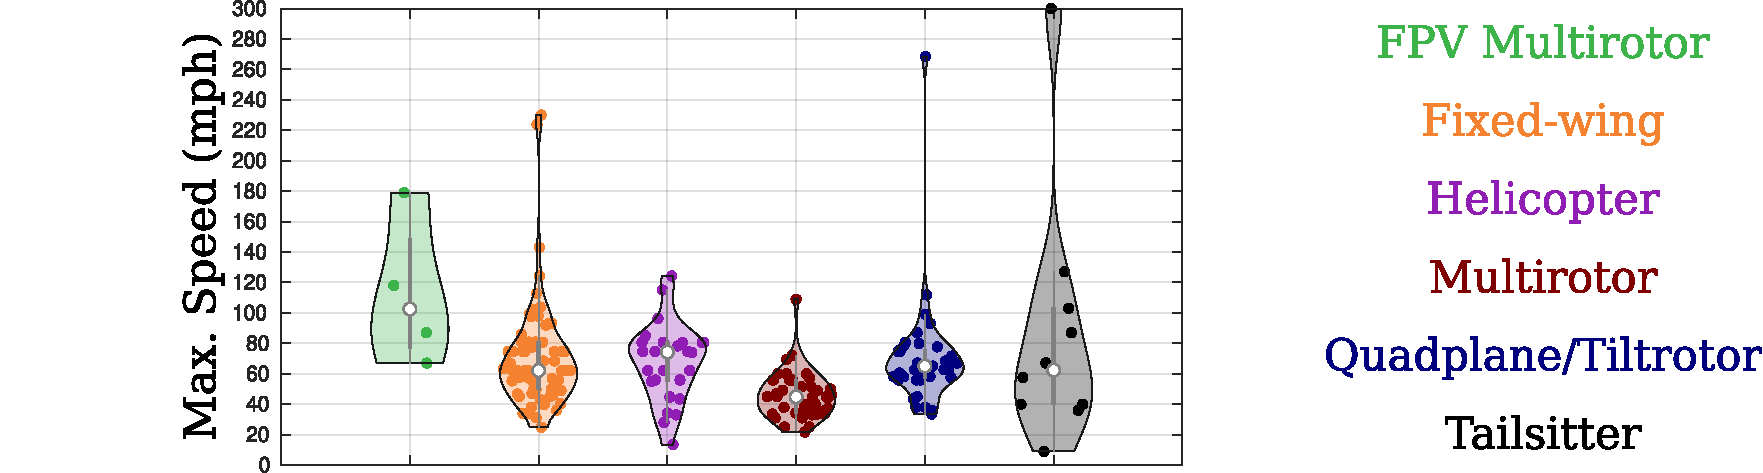
\includegraphics[width=\linewidth]{figs/misc/speed1.pdf}
            % \caption{Categorical UAV top speed \cite{kakavitsasSurvey}}
            \captionsetup{labelformat=empty}
            \caption{\cite{kakavitsasSurvey}}
        \end{figure}
    }
    \only<2>{
        \begin{figure}
            \centering
            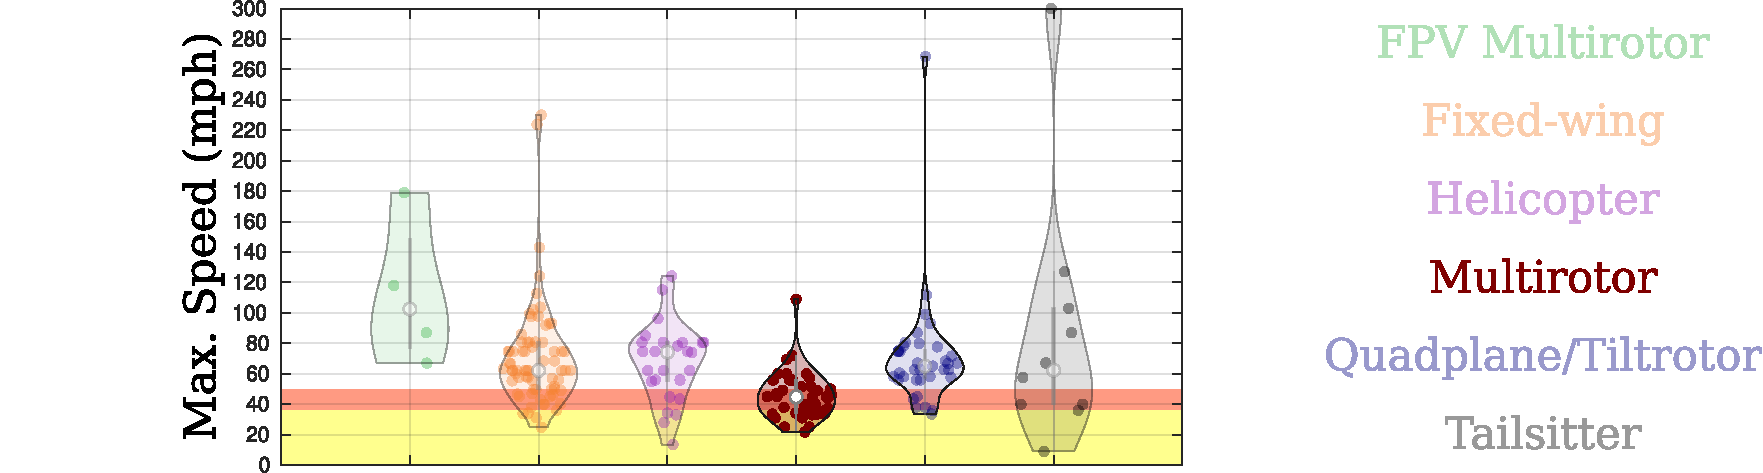
\includegraphics[width=\linewidth]{figs/misc/speed2.pdf}
            % \caption{Categorical UAV top speed \cite{kakavitsasSurvey}}
            \captionsetup{labelformat=empty}
            \caption{\cite{kakavitsasSurvey}}
        \end{figure}
    }
    \begin{columns}
        \column{0.7\textwidth}
            \vspace{-0.5cm}
            \only<1>{
                \begin{table}[h!]
                    \centering
                    \footnotesize{\begin{tabular}{p{2.2cm}p{2.2cm}p{2.2cm}}
                    \hline \hline
                     & Gust (mph) & Speed (mph) \\ \hline
                    Mean & 22 & 11.46 \\ 
                    Median & 21.3 & 10.8 \\ 
                    Max & 56.6 & 38.4 \\ \hline \hline
                    \end{tabular}}
                \end{table}
            }
            \only<2>{
                \begin{table}[h!]
                    \centering
                    \footnotesize{\begin{tabular}{p{2.2cm}p{2.2cm}p{2.2cm}}
                    \hline \hline
                     & Gust (mph) & Speed (mph) \\ \hline
                    Mean & 22 & 11.46 \\ 
                    Median & 21.3 & 10.8 \\ 
                    Max & \cellcolor[HTML]{ff9a82} 56.6 & \cellcolor[HTML]{ffff8e} 38.4 \\ \hline \hline
                    \end{tabular}}
                    % \scriptsize{\caption{Charlotte, NC windspeed and gust data for 2023 \cite{cltWind}}}
                \end{table}
            }
        \column{0.35\textwidth}
            % \begin{center}
            \small{Charlotte, NC wind speed and gust data for 2023-24 \cite{cltWind}}
            % \end{center}
    \end{columns}
    
\end{frame}

\begin{frame}{Thesis Statement \hfill 
\includegraphics[height=.5cm]{figs/uncc/whiteUNCCLogo.eps}}
    {Put your sample text here.  \emphPtGold{Emphasize points} with the commands defined in main.tex}
    \vspace{-0.2cm}
    Make a figure that defines all topics of your dissertation and ties in with the thesis statement at the top.
    \begin{figure}
        \centering
        \includegraphics[width=0.85\linewidth]{example-image-a}
    \end{figure}
\end{frame}



% Example slides
% --- --- --- --- --- --- --- --- --- --- --- 
% In the optional argument of the frame below, i.e. \begin{frame}{Title \hfill logo \hfill UNCC Logo}, add a logo for your section in place of the "figs/topic3White.pdf".  Make sure it has a transparent background, and that it uses white elements to ensure it's visible.

\section{Click2ExTable}
\begin{frame}{Example Multi-Slide Table and Equations\hfill 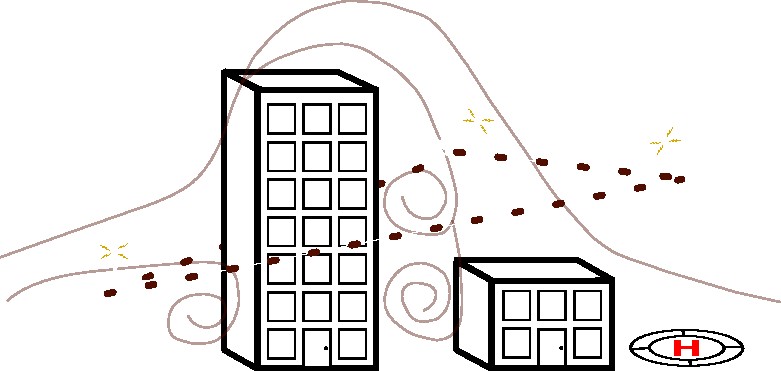
\includegraphics[height=.7cm]{figs/exTopicLogo.pdf} \;\;\;\;\; 
\includegraphics[height=.5cm]{figs/uncc/whiteUNCCLogo.eps}}
    \begin{columns}[T,onlytextwidth]
        \column{0.475\textwidth}
            \only<1-2>{
                In this work, we investigate the use of various feature spaces $F_{i}$ corresponding to respective feature vectors $\bm{x}_i$.  \\ \; \\
                These feature vectors contain some combination of
                \begin{itemize}
                    \item $\bm{r} = $ Locations of wind samples
                    \item $\rho(\bm{r}) , \nabla\rho(\bm{r})= $ SDF and gradient samples at $\bm{r}$
                    \item $\rho(\bm{r}+\bm{b}_{i}) , \nabla\rho(\bm{r}+\bm{b}_{i}) = $ SDF and gradient samples at $\bm{b}_{i}$ points surrounding $\bm{r}$
                \end{itemize}
            }
            \only<3>{
                Some kernels that are investigated with different levels of optimization include:
                \begin{itemize}
                    \item $\kappa_{1}$ - Grouped squared exponential
                        % \vspace{-0.65cm}
                        \begin{align*}
                            \kappa_{1} = &\kappa_{\text{sq}}(\bm{h},\bm{\theta}_{\text{sq},\bm{r}}) + \kappa_{\text{sq}}(\bm{h},\bm{\theta}_{\text{sq},\rho(\bm{r}),\nabla \rho(\bm{r})}) \\ &+ \sum_{i = 1}^{R} \kappa_{\text{sq}}(\bm{h},\bm{\theta}_{\text{sq},\rho(\bm{r}+\bm{b}_{i}),\nabla\rho(\bm{r}+\bm{b}_{i})}) 
                        \end{align*}
                \end{itemize}
            }
            \only<4>{
                Some kernels that are investigated with different levels of optimization include:
                \begin{itemize}
                    \item $\kappa_{1}$ - Grouped squared exponential
                    \item $\kappa_{2}$ - Standard squared exponential $\times$ coregion kernel \cite{bonilla2008, tipping1999}
                \end{itemize}
            }
            \only<5>{
                Some kernels that are investigated with different levels of optimization include:
                \begin{itemize}
                    \item $\kappa_{1}$ - Grouped squared exponential
                    \item $\kappa_{2}$ - Standard squared exponential $\times$ coregion kernel \cite{bonilla2008, tipping1999}
                    \item $\kappa_{3}$ - Standard squared exponential
                        % \vspace{-0.65cm}
                        \begin{align*}  
                            \kappa_{\text{sq}}(\bm{h},\;\bm{\theta}_{\text{sq}}) = \sigma^2 \text{exp}\left(-\frac{1}{2}\sum_{i=1}^{n}\left(\frac{h_i}{L_i}\right)^{2}\right)
                        \end{align*}
                \end{itemize}
            }
        \column{0.475\textwidth}
            \only<1>{
                Candidate vectors include:
                \vspace{-0.7cm}
                \begin{table}[h!]
                \centering
                \resizebox{\textwidth}{!}{%
                \begin{tabular}{ccccccc}
                \hline \hline
                No. & $\bm{r}$ & $\rho(\bm{r})$ & $\nabla \rho(\bm{r})$ & $\rho(\bm{r}+\bm{b}_{i,\dots,B})$ & $\nabla\rho(\bm{r}+\bm{b}_{i,\dots,B})$ \\ \hline
                $F_{1}$ & \cellcolor[HTML]{EFEFEF}\checkmark &  &  &  &   \\
                $F_{2}$ & \cellcolor[HTML]{EFEFEF}\checkmark & \cellcolor[HTML]{EFEFEF}\checkmark & \cellcolor[HTML]{EFEFEF}\checkmark &  &   \\
                $F_{3}$ & \cellcolor[HTML]{EFEFEF}\checkmark & \cellcolor[HTML]{EFEFEF}\checkmark & \cellcolor[HTML]{EFEFEF}\checkmark & \cellcolor[HTML]{EFEFEF}\checkmark & \cellcolor[HTML]{EFEFEF}\checkmark \\
                $F_{4}$ & \cellcolor[HTML]{EFEFEF}\checkmark & \cellcolor[HTML]{EFEFEF}\checkmark & \cellcolor[HTML]{EFEFEF}\checkmark & \cellcolor[HTML]{EFEFEF}\checkmark &   \\
                $F_{5}$ & \cellcolor[HTML]{EFEFEF}\checkmark & \cellcolor[HTML]{EFEFEF}\checkmark &  & \cellcolor[HTML]{EFEFEF}\checkmark &   \\
                $F_{6}$ & \cellcolor[HTML]{EFEFEF}\checkmark & \cellcolor[HTML]{EFEFEF}\checkmark &  &  &   \\
                $F_{7}$ & \cellcolor[HTML]{EFEFEF}\checkmark & \cellcolor[HTML]{EFEFEF}\checkmark & \cellcolor[HTML]{EFEFEF}\checkmark &  & \cellcolor[HTML]{EFEFEF}\checkmark  \\
                $F_{8}$ & \cellcolor[HTML]{EFEFEF}\checkmark &  & \cellcolor[HTML]{EFEFEF}\checkmark &  & \cellcolor[HTML]{EFEFEF}\checkmark  \\ \hline \hline
                \end{tabular}
                }
                \end{table}
            }
            \only<2>{
                Candidate vectors include:
                \vspace{-0.7cm}
                \begin{table}[h!]
                \centering
                \resizebox{\textwidth}{!}{%
                \begin{tabular}{ccccccc}
                \hline \hline
                No. & $\bm{r}$ & $\rho(\bm{r})$ & $\nabla \rho(\bm{r})$ & $\rho(\bm{r}+\bm{b}_{i,\dots,B})$ & $\nabla\rho(\bm{r}+\bm{b}_{i,\dots,B})$ \\ \hline
                $F_{1}$ & \cellcolor[HTML]{EFEFEF}\checkmark &  &  &  &   \\
                $F_{2}$ & \cellcolor[HTML]{EFEFEF}\checkmark & \cellcolor[HTML]{EFEFEF}\checkmark & \cellcolor[HTML]{EFEFEF}\checkmark &  &   \\
                $F_{3}$ & \cellcolor[HTML]{EFEFEF}\checkmark & \cellcolor[HTML]{EFEFEF}\checkmark & \cellcolor[HTML]{EFEFEF}\checkmark & \cellcolor[HTML]{EFEFEF}\checkmark & \cellcolor[HTML]{EFEFEF}\checkmark \\
                $F_{4}$ & \cellcolor[HTML]{EFEFEF}\checkmark & \cellcolor[HTML]{EFEFEF}\checkmark & \cellcolor[HTML]{EFEFEF}\checkmark & \cellcolor[HTML]{EFEFEF}\checkmark &   \\
                $F_{5}$ & \cellcolor[HTML]{EFEFEF}\checkmark & \cellcolor[HTML]{EFEFEF}\checkmark &  & \cellcolor[HTML]{EFEFEF}\checkmark &   \\
                $F_{6}$ & \cellcolor[HTML]{EFEFEF}\checkmark & \cellcolor[HTML]{EFEFEF}\checkmark &  &  &   \\
                $F_{7}$ & \cellcolor[HTML]{EFEFEF}\checkmark & \cellcolor[HTML]{EFEFEF}\checkmark & \cellcolor[HTML]{EFEFEF}\checkmark &  & \cellcolor[HTML]{EFEFEF}\checkmark  \\
                $F_{8}$ & \cellcolor[HTML]{EFEFEF}\checkmark &  & \cellcolor[HTML]{EFEFEF}\checkmark &  & \cellcolor[HTML]{EFEFEF}\checkmark  \\ \hline \hline
                \end{tabular}
                }
                \end{table}
            }
            \only<3>{
                Candidate vectors include:
                \vspace{-0.7cm}
                \begin{table}[h!]
                \centering
                \resizebox{\textwidth}{!}{%
                \begin{tabular}{ccccccc}
                \hline \hline
                No. & $\bm{r}$ & $\rho(\bm{r})$ & $\nabla \rho(\bm{r})$ & $\rho(\bm{r}+\bm{b}_{i,\dots,B})$ & $\nabla\rho(\bm{r}+\bm{b}_{i,\dots,B})$ \\ \hline
                $F_{1}$ & \cellcolor[HTML]{EFEFEF}\checkmark &  &  &  &   \\
                $F_{2}$ & \cellcolor[HTML]{EFEFEF}\checkmark & \cellcolor[HTML]{EFEFEF}\checkmark & \cellcolor[HTML]{EFEFEF}\checkmark &  &   \\
                $F_{3}$ \cellcolor{unccGoldOpaque} & \cellcolor[HTML]{EFEFEF}\checkmark & \cellcolor[HTML]{EFEFEF}\checkmark & \cellcolor[HTML]{EFEFEF}\checkmark & \cellcolor[HTML]{EFEFEF}\checkmark & \cellcolor[HTML]{EFEFEF}\checkmark \\
                $F_{4}$ & \cellcolor[HTML]{EFEFEF}\checkmark & \cellcolor[HTML]{EFEFEF}\checkmark & \cellcolor[HTML]{EFEFEF}\checkmark & \cellcolor[HTML]{EFEFEF}\checkmark &   \\
                $F_{5}$ & \cellcolor[HTML]{EFEFEF}\checkmark & \cellcolor[HTML]{EFEFEF}\checkmark &  & \cellcolor[HTML]{EFEFEF}\checkmark &   \\
                $F_{6}$ & \cellcolor[HTML]{EFEFEF}\checkmark & \cellcolor[HTML]{EFEFEF}\checkmark &  &  &   \\
                $F_{7}$ & \cellcolor[HTML]{EFEFEF}\checkmark & \cellcolor[HTML]{EFEFEF}\checkmark & \cellcolor[HTML]{EFEFEF}\checkmark &  & \cellcolor[HTML]{EFEFEF}\checkmark  \\
                $F_{8}$ & \cellcolor[HTML]{EFEFEF}\checkmark &  & \cellcolor[HTML]{EFEFEF}\checkmark &  & \cellcolor[HTML]{EFEFEF}\checkmark  \\ \hline \hline
                \end{tabular}
                }
                \end{table}
                \textcolor{unccGold}{Gaussian Process Regression (GPR)}\\
                \textcolor{unccClayRed}{Variational GPR (VGP)}
            }
            \only<4>{
                Candidate vectors include:
                \vspace{-0.7cm}
                \begin{table}[h!]
                \centering
                \resizebox{\textwidth}{!}{%
                \begin{tabular}{ccccccc}
                \hline \hline
                No. & $\bm{r}$ & $\rho(\bm{r})$ & $\nabla \rho(\bm{r})$ & $\rho(\bm{r}+\bm{b}_{i,\dots,B})$ & $\nabla\rho(\bm{r}+\bm{b}_{i,\dots,B})$ \\ \hline
                $F_{1}$ \cellcolor{unccclayRedOpaque}& \cellcolor[HTML]{EFEFEF}\checkmark &  &  &  &   \\
                $F_{2}$ & \cellcolor[HTML]{EFEFEF}\checkmark & \cellcolor[HTML]{EFEFEF}\checkmark & \cellcolor[HTML]{EFEFEF}\checkmark &  &   \\
                $F_{3}$ & \cellcolor[HTML]{EFEFEF}\checkmark & \cellcolor[HTML]{EFEFEF}\checkmark & \cellcolor[HTML]{EFEFEF}\checkmark & \cellcolor[HTML]{EFEFEF}\checkmark & \cellcolor[HTML]{EFEFEF}\checkmark \\
                $F_{4}$ & \cellcolor[HTML]{EFEFEF}\checkmark & \cellcolor[HTML]{EFEFEF}\checkmark & \cellcolor[HTML]{EFEFEF}\checkmark & \cellcolor[HTML]{EFEFEF}\checkmark &   \\
                $F_{5}$ & \cellcolor[HTML]{EFEFEF}\checkmark & \cellcolor[HTML]{EFEFEF}\checkmark &  & \cellcolor[HTML]{EFEFEF}\checkmark &   \\
                $F_{6}$ & \cellcolor[HTML]{EFEFEF}\checkmark & \cellcolor[HTML]{EFEFEF}\checkmark &  &  &   \\
                $F_{7}$ & \cellcolor[HTML]{EFEFEF}\checkmark & \cellcolor[HTML]{EFEFEF}\checkmark & \cellcolor[HTML]{EFEFEF}\checkmark &  & \cellcolor[HTML]{EFEFEF}\checkmark  \\
                $F_{8}$ & \cellcolor[HTML]{EFEFEF}\checkmark &  & \cellcolor[HTML]{EFEFEF}\checkmark &  & \cellcolor[HTML]{EFEFEF}\checkmark  \\ \hline \hline
                \end{tabular}
                }
                \end{table}
                \textcolor{unccGold}{Gaussian Process Regression (GPR)}\\
                \textcolor{unccClayRed}{Variational GPR (VGP)}
            }
            \only<5>{
                Candidate vectors include:
                \vspace{-0.7cm}
                \begin{table}[h!]
                \centering
                \resizebox{\textwidth}{!}{%
                \begin{tabular}{ccccccc}
                \hline \hline
                No. & $\bm{r}$ & $\rho(\bm{r})$ & $\nabla \rho(\bm{r})$ & $\rho(\bm{r}+\bm{b}_{i,\dots,B})$ & $\nabla\rho(\bm{r}+\bm{b}_{i,\dots,B})$ \\ \hline
                $F_{1}$ \cellcolor{unccGoldOpaque}& \cellcolor[HTML]{EFEFEF}\checkmark &  &  &  &   \\
                $F_{2}$ \cellcolor{unccGoldOpaque}& \cellcolor[HTML]{EFEFEF}\checkmark & \cellcolor[HTML]{EFEFEF}\checkmark & \cellcolor[HTML]{EFEFEF}\checkmark &  &   \\
                $F_{3}$ \cellcolor{unccGoldOpaque}& \cellcolor[HTML]{EFEFEF}\checkmark & \cellcolor[HTML]{EFEFEF}\checkmark & \cellcolor[HTML]{EFEFEF}\checkmark & \cellcolor[HTML]{EFEFEF}\checkmark & \cellcolor[HTML]{EFEFEF}\checkmark \\
                $F_{4}$ \cellcolor{unccGoldOpaque}& \cellcolor[HTML]{EFEFEF}\checkmark & \cellcolor[HTML]{EFEFEF}\checkmark & \cellcolor[HTML]{EFEFEF}\checkmark & \cellcolor[HTML]{EFEFEF}\checkmark &   \\
                $F_{5}$ \cellcolor{unccGoldOpaque}& \cellcolor[HTML]{EFEFEF}\checkmark & \cellcolor[HTML]{EFEFEF}\checkmark &  & \cellcolor[HTML]{EFEFEF}\checkmark &   \\
                $F_{6}$ \cellcolor{unccGoldOpaque}& \cellcolor[HTML]{EFEFEF}\checkmark & \cellcolor[HTML]{EFEFEF}\checkmark &  &  &   \\
                $F_{7}$ \cellcolor{unccGoldOpaque}& \cellcolor[HTML]{EFEFEF}\checkmark & \cellcolor[HTML]{EFEFEF}\checkmark & \cellcolor[HTML]{EFEFEF}\checkmark &  & \cellcolor[HTML]{EFEFEF}\checkmark  \\
                $F_{8}$ \cellcolor{unccGoldOpaque}& \cellcolor[HTML]{EFEFEF}\checkmark &  & \cellcolor[HTML]{EFEFEF}\checkmark &  & \cellcolor[HTML]{EFEFEF}\checkmark  \\ \hline \hline
                \end{tabular}
                }
                \end{table}
                \textcolor{unccGold}{Gaussian Process Regression (GPR)}\\
                \textcolor{unccClayRed}{Variational GPR (VGP)}
            }
    \end{columns}
    
\end{frame}
% In the optional argument of the frame below, i.e. \begin{frame}{Title \hfill logo \hfill UNCC Logo}, add a logo for your section in place of the "figs/topic3White.pdf".  Make sure it has a transparent background, and that it uses white elements to ensure it's visible.

\section{Click2ExAnimation}
\begin{frame}{Example Animation \hfill 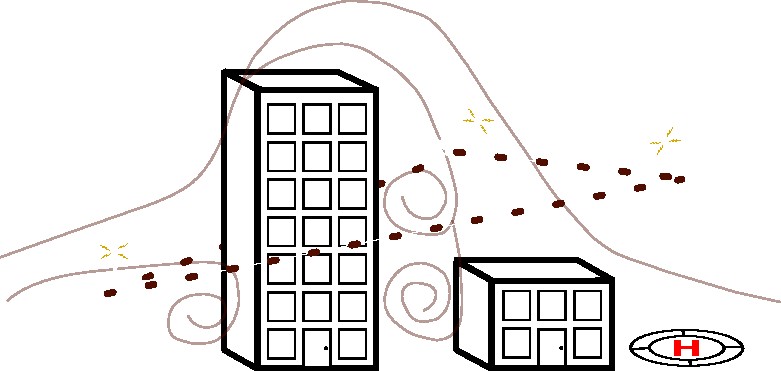
\includegraphics[height=.7cm]{figs/exTopicLogo.pdf} \;\;\;\;\; 
\includegraphics[height=.5cm]{figs/uncc/whiteUNCCLogo.eps}}
    These animations only really work when viewed in Adobe reader.  Adobe reader has a presentation mode, and during the presentation, you just use the controls under the animation frame to play the animation.

    \begin{columns}[T,onlytextwidth]
        \column{0.8\textwidth}
            \animategraphics[loop,controls,width=\linewidth]{70}{figs/gpAnimation/gpAnimationFrame-}{0}{85}
        \column{0.2\textwidth}
            \begin{align*}
                L &= 1.5 \text{ m} \\
                \sigma^{2} &= 4 \text{ m}^{2}\\
                \sigma_{n}^{2} &= 0.6 \; (\text{m/s})^{2} \\
                \mu_{w} &= -8 \text{ m/s}
            \end{align*}
    \end{columns}
\end{frame}


% Chapter 3: ADD YOUR CH3 NAME HERE
% --- --- --- --- --- --- --- --- --- --- --- 
% \include{sections/ch3Section}

% Chapter 4: ADD YOUR CH4 NAME HERE
% --- --- --- --- --- --- --- --- --- --- --- 
% \include{sections/ch4Section}

% Chapter 5: ADD YOUR CH5 NAME HERE
% --- --- --- --- --- --- --- --- --- --- --- 
% \include{sections/ch5Section}

% etc chapters as needed


% Chapter N: Conclusion 
% --- --- --- --- --- --- --- --- --- --- --- 
% \include{sections/conclusions}

% --- References ---
\setbeamertemplate{frametitle continuation}{}
\begin{frame}[allowframebreaks,noframenumbering]{References}
    \bibliography{refs}
    \bibliographystyle{apalike}
\end{frame}

% Appendix/backup slides
% --- --- --- --- --- --- --- --- --- --- --- 
\appendix
%%%%%%%%%%%%%%%%%%%%%%%%%%%%%%%%%%%%%%%%%%%%%%%%%%%%%%%%%%%%%%%%%%%%%%%%%%%%%%%
%%%%%%%%%%%%%%%%%%%%%%%% Introduction appendix slides %%%%%%%%%%%%%%%%%%%%%%%%
%%%%%%%%%%%%%%%%%%%%%%%%%%%%%%%%%%%%%%%%%%%%%%%%%%%%%%%%%%%%%%%%%%%%%%%%%%%%%%%
\section{\hyperlink{sec:intro}{Example Appendix Slide}}\label{apdx:intro}
\begin{frame}{Introduction \hfill 
\includegraphics[height=.5cm]{figs/uncc/whiteUNCCLogo.eps}}
    Introduction appendix slides
\end{frame}

\begin{frame}{UAV Classifications \hfill 
\includegraphics[height=.5cm]{figs/uncc/whiteUNCCLogo.eps}}
    % \only<1>{
    \begin{table}[h!]
        \centering
        % \renewcommand{\arraystretch}{1.25}
        \small{\caption{U.S. Department of Defense UAS classifications. \cite{miller2021counter}.}}
        \begin{tabular}{|p{2.2cm}|p{2.2cm}|p{3cm}|p{3cm}|}
        \hline 
        \footnotesize{UAS Group} & \footnotesize{Maximum takeoff weight (lbs) (MTOW)} & \footnotesize{Nominal operating altitude (ft)} & \footnotesize{Speed} \newline \scriptsize{(knots) [mph]} 
            \\  \hline
            Group 1 & 0$-$20 & $<$ 1,200 AGL & 100 [115]
            \\ \hline
            Group 2 & 21$-$55 & $<$ 3,500 AGL & $<$ 250 [289]
            \\ \hline
            Group 3 & $<$ 1,320 & $<$ FL 18,000 & $<$ 250 [289]
            \\ \hline
            Group 4 & $<$ 1,320 & $<$ FL 18,000 & Any airspeed
            \\ \hline
            Group 5 & $<$ 1,320 & $>$ FL 18,000 & Any airspeed\\
            \hline
        \end{tabular}
        \label{tab:UAS_group}
    \end{table}
\end{frame}


\end{document}